%%%%%%%%%%%%%%%%%%%%%%%%%%%%%%%%%%%%%%%%%
% Beamer Presentation
% LaTeX Template
% Version 1.0 (10/11/12)
%
% This template has been downloaded from:
% http://www.LaTeXTemplates.com
%
% License:
% CC BY-NC-SA 3.0 (http://creativecommons.org/licenses/by-nc-sa/3.0/)
%
%%%%%%%%%%%%%%%%%%%%%%%%%%%%%%%%%%%%%%%%%

%----------------------------------------------------------------------------------------
%	PACKAGES AND THEMES
%----------------------------------------------------------------------------------------

\documentclass{beamer}
\usepackage[spanish]{babel}
\usepackage[T1]{fontenc}
\usepackage[utf8]{inputenc}
\usepackage{graphicx,amssymb,amsmath,indentfirst,upref}
%\usepackage[ansinew]{inputenc}
\usepackage{latexsym,fancyhdr,supertabular,colortbl}
\usepackage[spanish]{babel}
\usepackage{colortbl}
\usepackage{fancybox}
\usepackage{csquotes}
\usetheme{Madrid}
\usecolortheme{seahorse}
\usecolortheme{rose}
\usefonttheme[onlylarge]{structuresmallcapsserif}
\usefonttheme[onlysmall]{structurebold}
\setbeamerfont{title}{shape=\itshape,family=\rmfamily}
\setbeamertemplate{footline}{\insertpagenumber}
\mode<presentation> {
\usepackage{xcolor}
% The Beamer class comes with a number of default slide themes
% which change the colors and layouts of slides. Below this is a list
% of all the themes, uncomment each in turn to see what they look like.
%originalmente Madrid
%\usetheme{default}
%\usetheme{AnnArbor}
%\usetheme{Antibes}
%\usetheme{Bergen}
%\usetheme{Berkeley}
%\usetheme{Berlin}
%\usetheme{Boadilla}
%\usetheme{CambridgeUS}
%\usetheme{Copenhagen}
%\usetheme{Darmstadt}
%\usetheme{Dresden}
%\usetheme{Frankfurt}
%\usetheme{Goettingen}
%\usetheme{Hannover}
%\usetheme{Ilmenau}
%\usetheme{JuanLesPins}
%\usetheme{Luebeck}
%\usetheme{Madrid}
%\usetheme{Malmoe}
%\usetheme{Marburg}
%\usetheme{Montpellier}
%\usetheme{PaloAlto}
%\usetheme{Pittsburgh}
%\usetheme{Rochester}
%\usetheme{Singapore}
%\usetheme{Szeged}
%\usetheme{Warsaw}

% As well as themes, the Beamer class has a number of color themes
% for any slide theme. Uncomment each of these in turn to see how it
% changes the colors of your current slide theme.
%Originalmente no hab�a ninguno activo
%\usecolortheme{albatross}
%\usecolortheme{beaver}
%\usecolortheme{beetle}
%\usecolortheme{crane}
%\usecolortheme{dolphin}
%\usecolortheme{dove}
%\usecolortheme{fly}
%\usecolortheme{lily}
%\usecolortheme{orchid}
\usecolortheme{rose}
%\usecolortheme{seagull}
\usecolortheme{seahorse}
%\usecolortheme{whale}
%\usecolortheme{wolverine}

%\setbeamertemplate{footline} % To remove the footer line in all slides uncomment this line
\setbeamertemplate{footline}[page number] % To replace the footer line in all slides with a simple slide count uncomment this line

\setbeamertemplate{navigation symbols}{} % To remove the navigation symbols from the bottom of all slides uncomment this line
}

\usepackage{graphicx} % Allows including images
\usepackage{booktabs} % Allows the use of \toprule, \midrule and \bottomrule in tables

%----------------------------------------------------------------------------------------
%	TITLE PAGE
%----------------------------------------------------------------------------------------

\title[Short title]{Introduction to the Course Statistical Data Analysis} % The short title appears at the bottom of every slide, the full title is only on the title page

\author{} % Your name
\institute[] % Your institution as it will appear on the bottom of every slide, may be shorthand to save space
{
 \\ % Your institution for the title page
\medskip
\textit{} % Your email address
}
\date{} % Date, can be changed to a custom date

\begin{document}
\decimalpoint
\begin{frame}
\titlepage % Print the title page as the first slide
\end{frame}

% Tabla de contenidos
\begin{frame}
\frametitle{Contents} % Table of contents slide, comment this block out to remove it
\tableofcontents % Throughout your presentation, if you choose to use \section{} and \subsection{} commands, these will automatically be printed on this slide as an overview of your presentation
\end{frame}

%----------------------------------------------------------------------------------------
%	PRESENTATION SLIDES
%----------------------------------------------------------------------------------------
\section{Main Objectives}
%----------------------------------------------------------------------------------------
\begin{frame}
\frametitle{Main Objectives}
\begin{itemize}
\item That students begin to develop the skills to be able to organize, 
analyse and interpret data.  
\item To gain insights into data through computation, statistics and 
visualization. 
\item To work on the ability to take data- to be able to understand it, 
to process it, to extract value from it, to visualize it, to communicate conclusions.\\[15pt]
\end{itemize}
\begin{displayquote}
\textcolor{blue}{Statistics has been the most successful information science. Those who ignore
Statistics are condemned to re-invent it. \\ - Brad Efron, 1997}
\end{displayquote}
\end{frame}
%--------------------------------------------------------
\begin{frame}
\frametitle{Main Objectives}
\begin{itemize}
\item To become informed consumers of the statistical methods/models 
presented in this course. \\[30pt]

\item To be able to properly obtain and use the statistical methods presented 
in this course.
\end{itemize}

\end{frame}
%----------------------------------------------
\section{Data Analysis}
%----------------------------------------------
\begin{frame}
\frametitle{Data Analysis}
The process of data analysis is a creative one, it can't be generalized and written down as a recipe to follow. It is not magically finding nuggets of information in a data set. It is, by nature, an amorphous and time consuming-process, full of open-ended questions and following up leads that often reach dead-ends. \\[20pt] 
\begin{displayquote}
\textcolor{blue}{How can one effectively generalize across many different data analyses, each of which has important unique aspects?} \\[3pt]
The Art of Data Science, R.D. Peng, E. Matsui
\end{displayquote} 
\vspace*{.5cm}
\begin{displayquote}
\textcolor{blue}{We think that good analysis depends not only on clear thinking but also on substantive knowledge. Mere numerology will not do, nor is there a good cookbook.} \\[3pt]
David Freedman, 1987
\end{displayquote} 
\end{frame}
%----------------------------------------------
\begin{frame}
\frametitle{Data Analysis}
Ultimately, a data analyst must find a way to assemble all of the tools and apply them to data to answer a relevant question—a question of interest to people. \\[10pt]

What should be described as data analysis is not a specific “formula” for data analysis—something like “apply this method and then run that test”— but rather is a general process that can be applied in a variety of situations. \\[10pt]

The starting point of any data analysis should be a set of questions about the data set
you want to answer. Data analysis is a question-driven process. The starting point is a 
\textcolor{blue}{research question of interest}. 

% You get the basics and fill in the gaps with experience. We can learn a bunch of tools and a general process but experience is the one that gives shape to this set of tools, to this knowledge
\end{frame}
%----------------------------------------------
\begin{frame}
\frametitle{Data Analysis: research questions}
Starting Point: it is usually some research question. Because \textit{doing data science} is basically leverage data to answer questions.\\[15pt]
Some examples might be: \\[10pt]
\begin{itemize}
\item A researcher is interested in understanding the effect of smoking and weight upon the resting pulse (Low/High).\\[15pt]
\item A dietician is interested in studying the general trends in the composition of cereals.
\begin{itemize}
\item What ingredients best predict the amount of calories a cereal contain?
\item Does service size play a role in the amount of calories?
\item Are the trends in predicting calories the same across manufacturers?
\end{itemize}
\end{itemize}
%\begin{itemize}
%\item Why are we losing money?
%\item Who uses / buys our products?
%\item How can we make ore money?
%\item How we do compare with our competitors?
%\item When something happened?
%\end{itemize}
\end{frame}
%--------------------------------------------
\begin{frame}
\frametitle{Data Analysis: research questions}
\begin{itemize}
\item Has there been global warming over the past decade?\\[15pt]
\item Is having the death penalty available for punishment associated with a reduction in violent crime?\\[15pt]
\item Does student performance in class depend on the amount of money spent per student, the size of the classes or the teachers' salaries?
\end{itemize}
\end{frame}
%--------------------------------------------- 
% Everything is centered around DATA, everything starts with data, but the analyst perspective is not the only one that matters
% From the analyst perspective, for instance, and reading this piece of news we might be interested in addressing the following question
\begin{frame}
\frametitle{Data Analysis}
NBA Data 2016-2017. Regular Season. 

\begin{center}
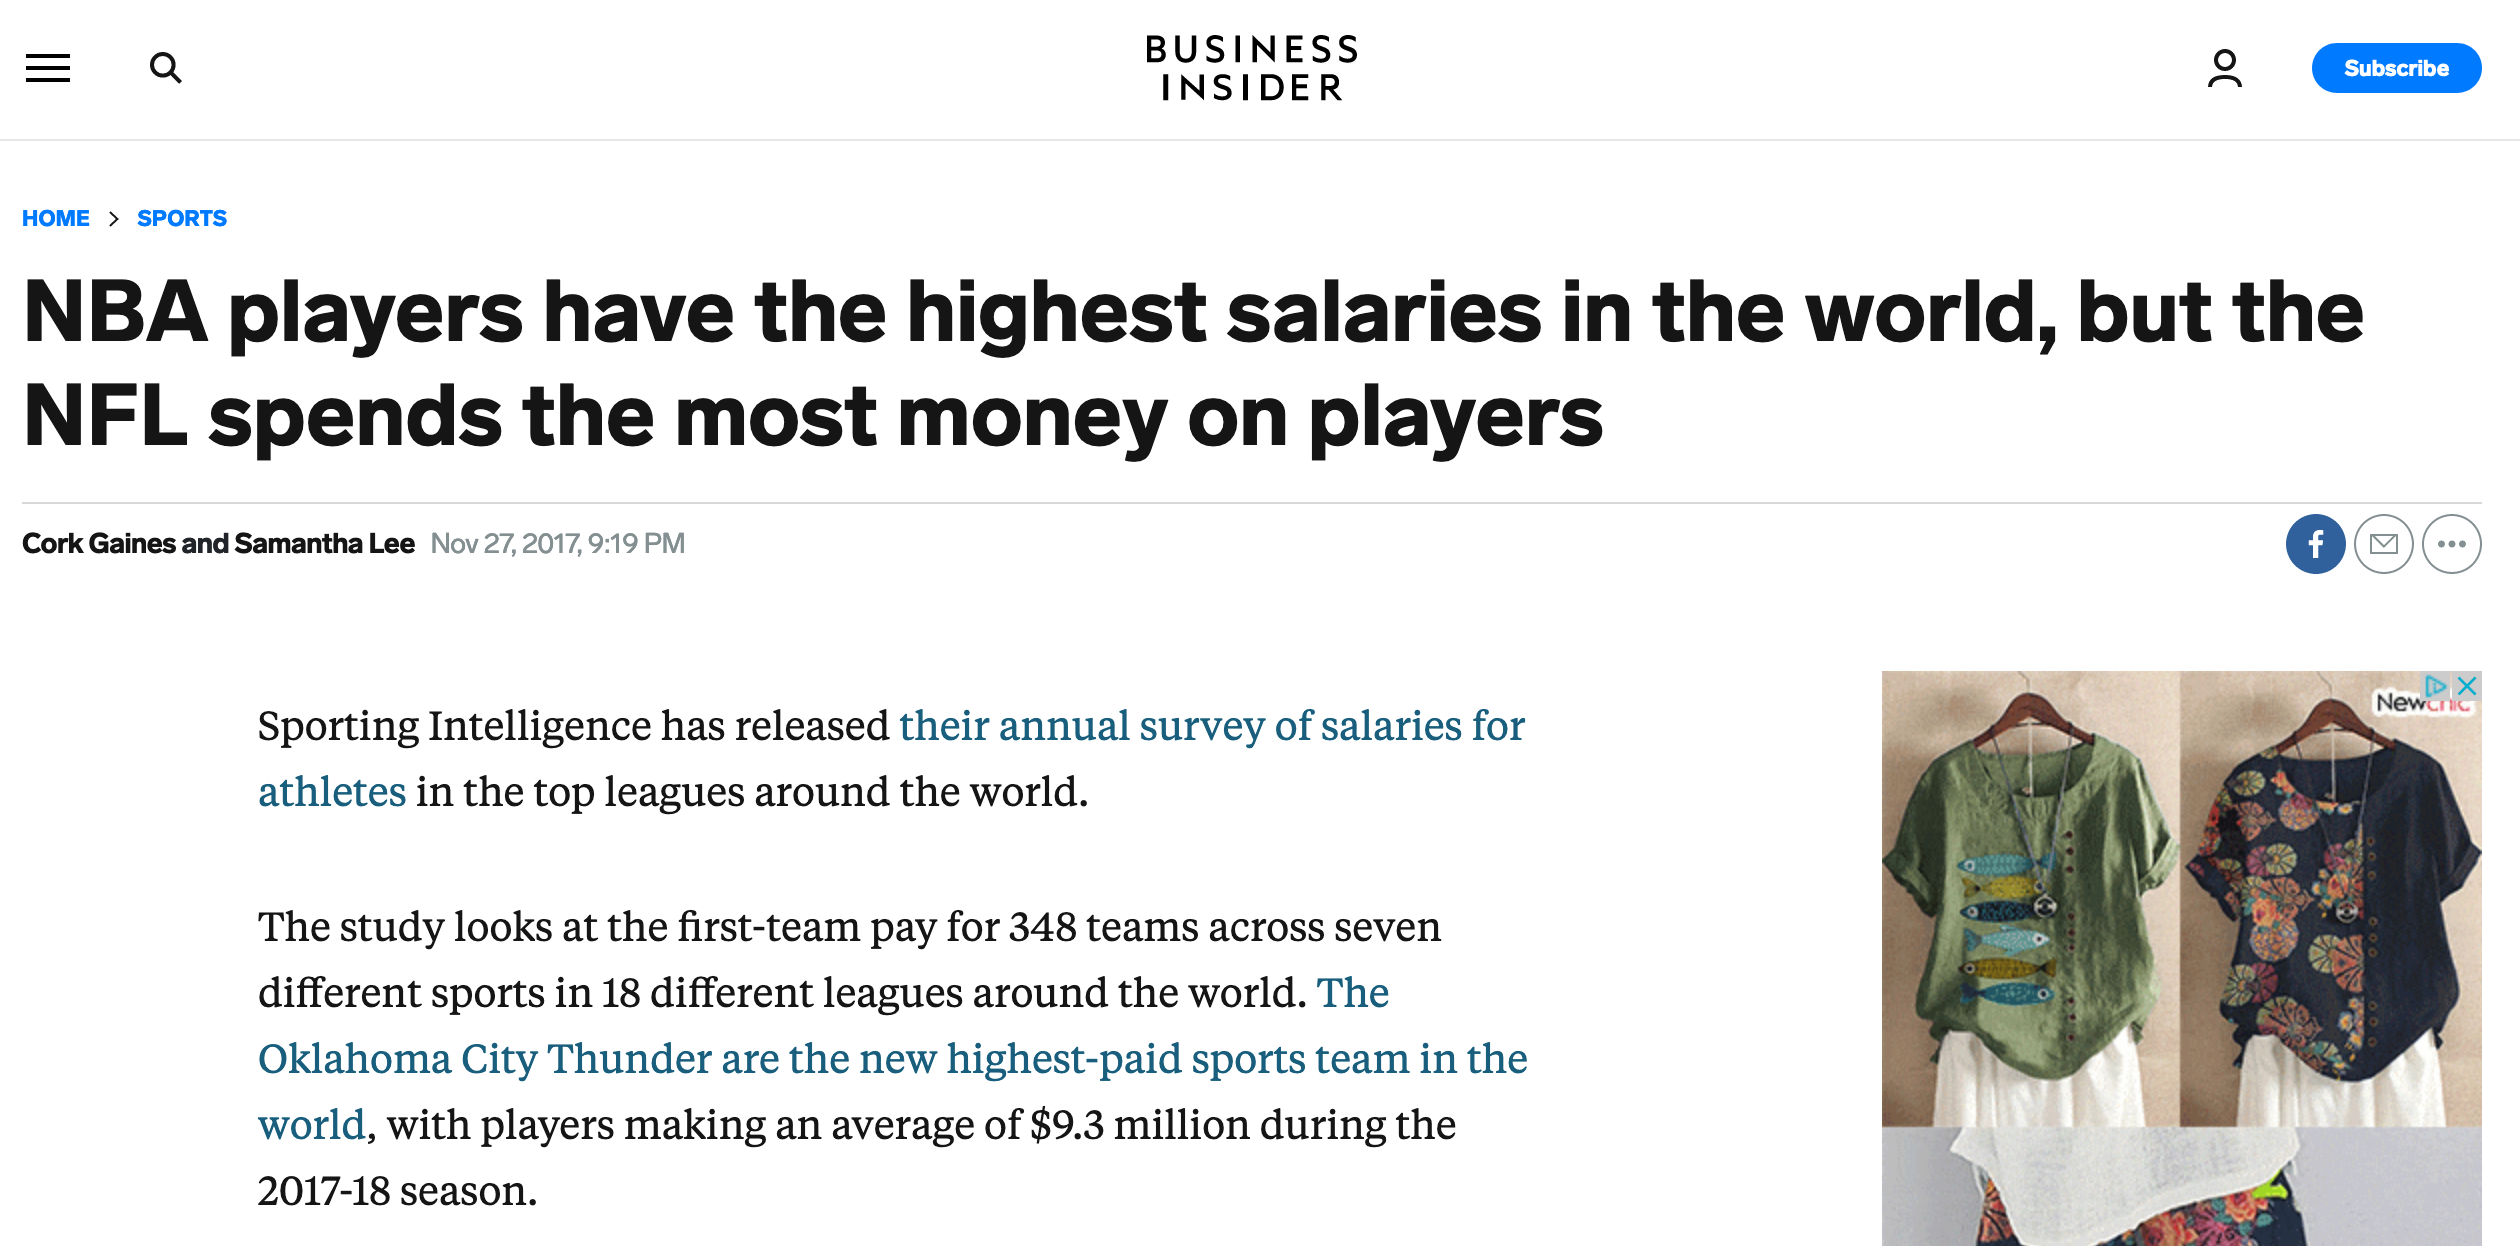
\includegraphics[scale=0.25]{./figures/sports.png}
\end{center}

\end{frame}
%--------------------------------------------
\begin{frame}
\frametitle{Data Analysis}
% and with our analyst perspective we can think of a model
Research Question: The more scored points, the higher the salary? \\[10pt]

How do analysts and scientists think about the data?

\begin{center}
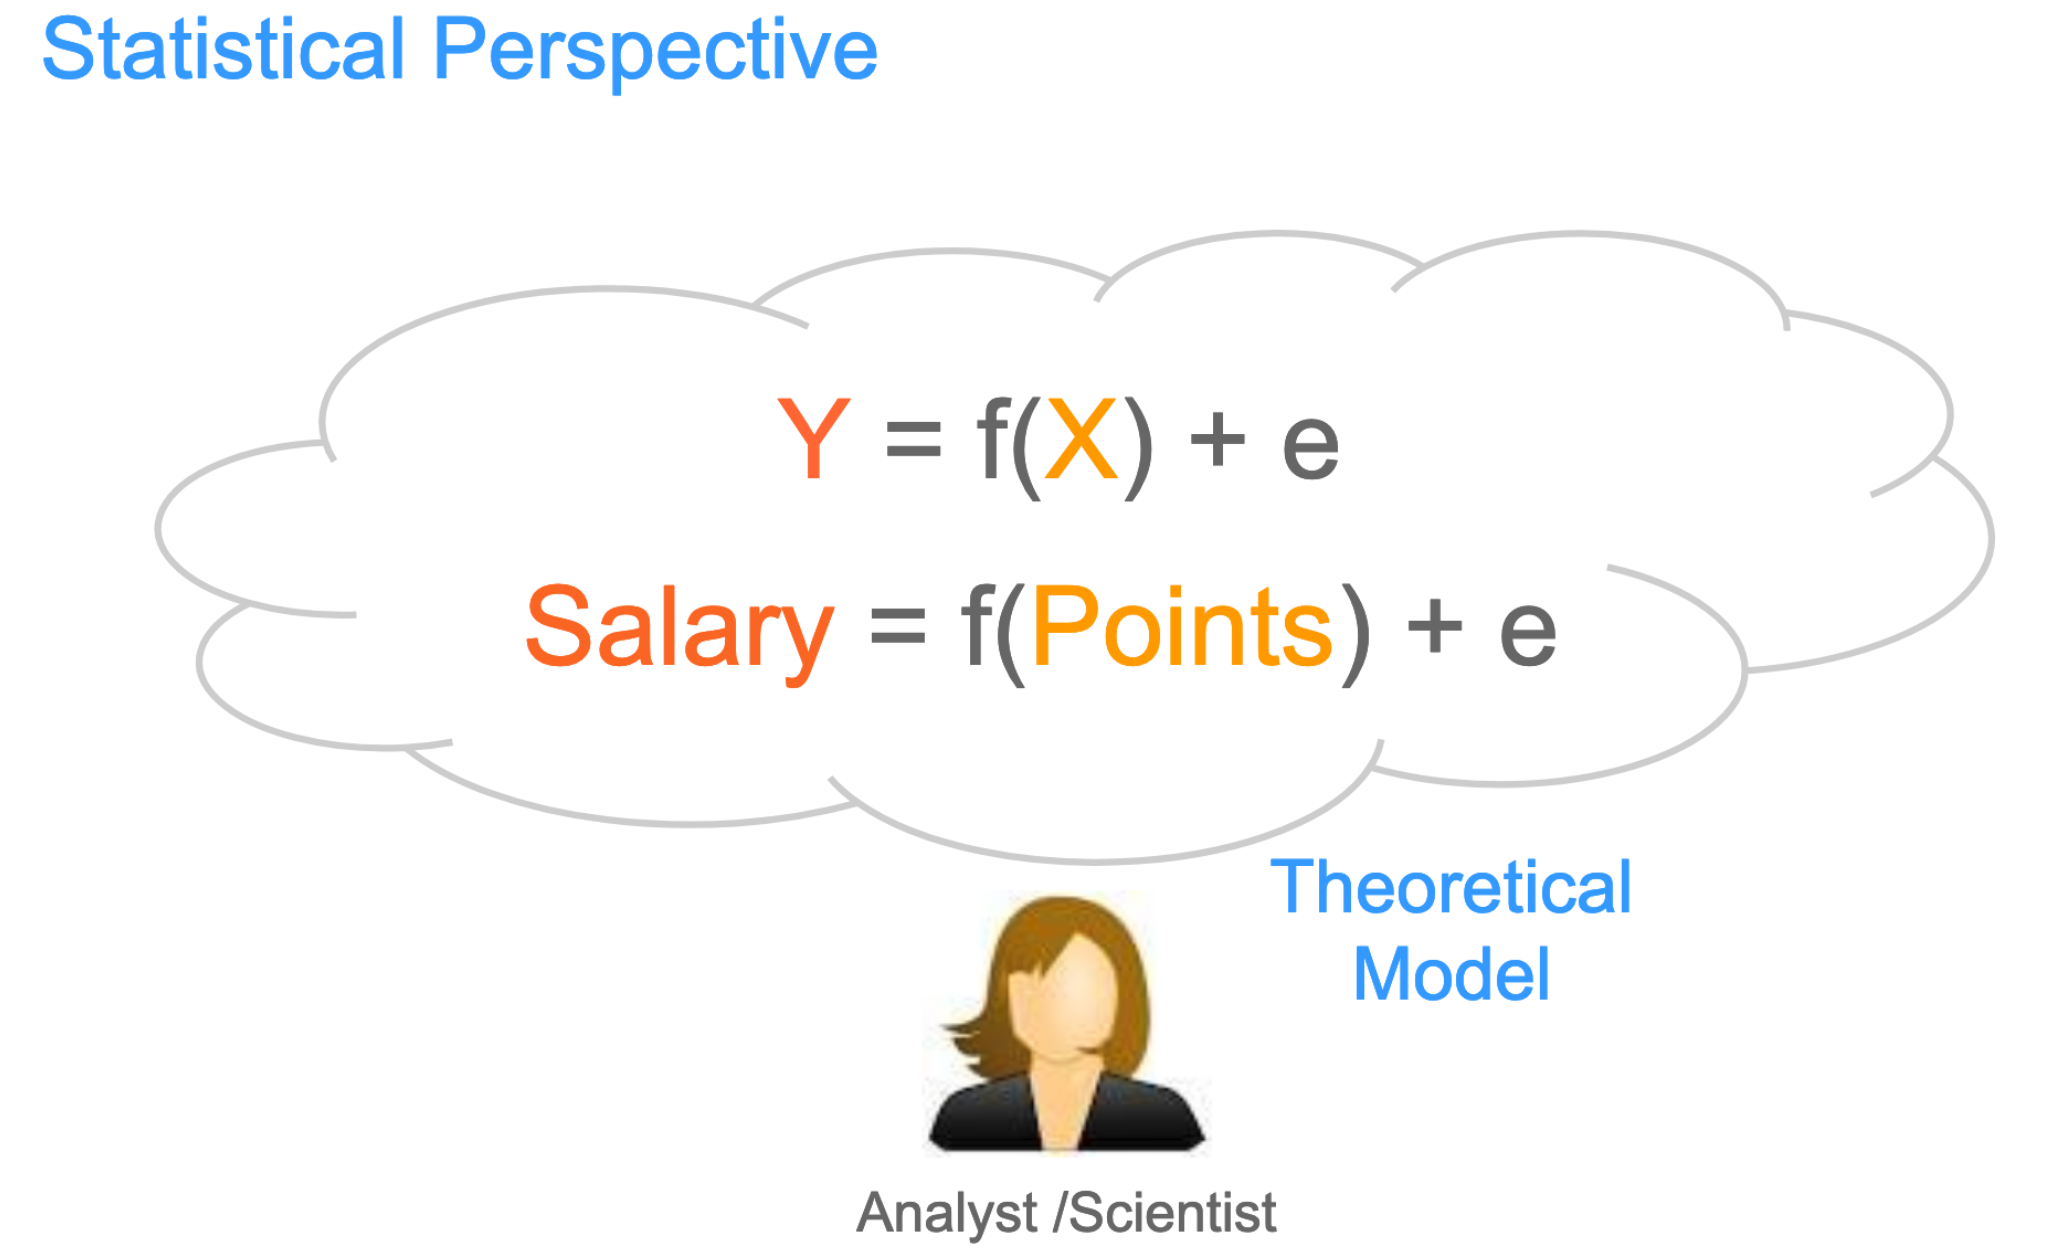
\includegraphics[scale=0.25]{sports_1.png}
\end{center}

\end{frame}
%--------------------------------------------
\begin{frame}
% But I don't want you to forget that there's a wider picture, besides data analysis there is a lot going on surrounding the data itself, from data collection, storage,
% technologies to 
\frametitle{The Big Picture}
What about the data? How do computers treat data? How do programming languages handle data? 

\begin{center}
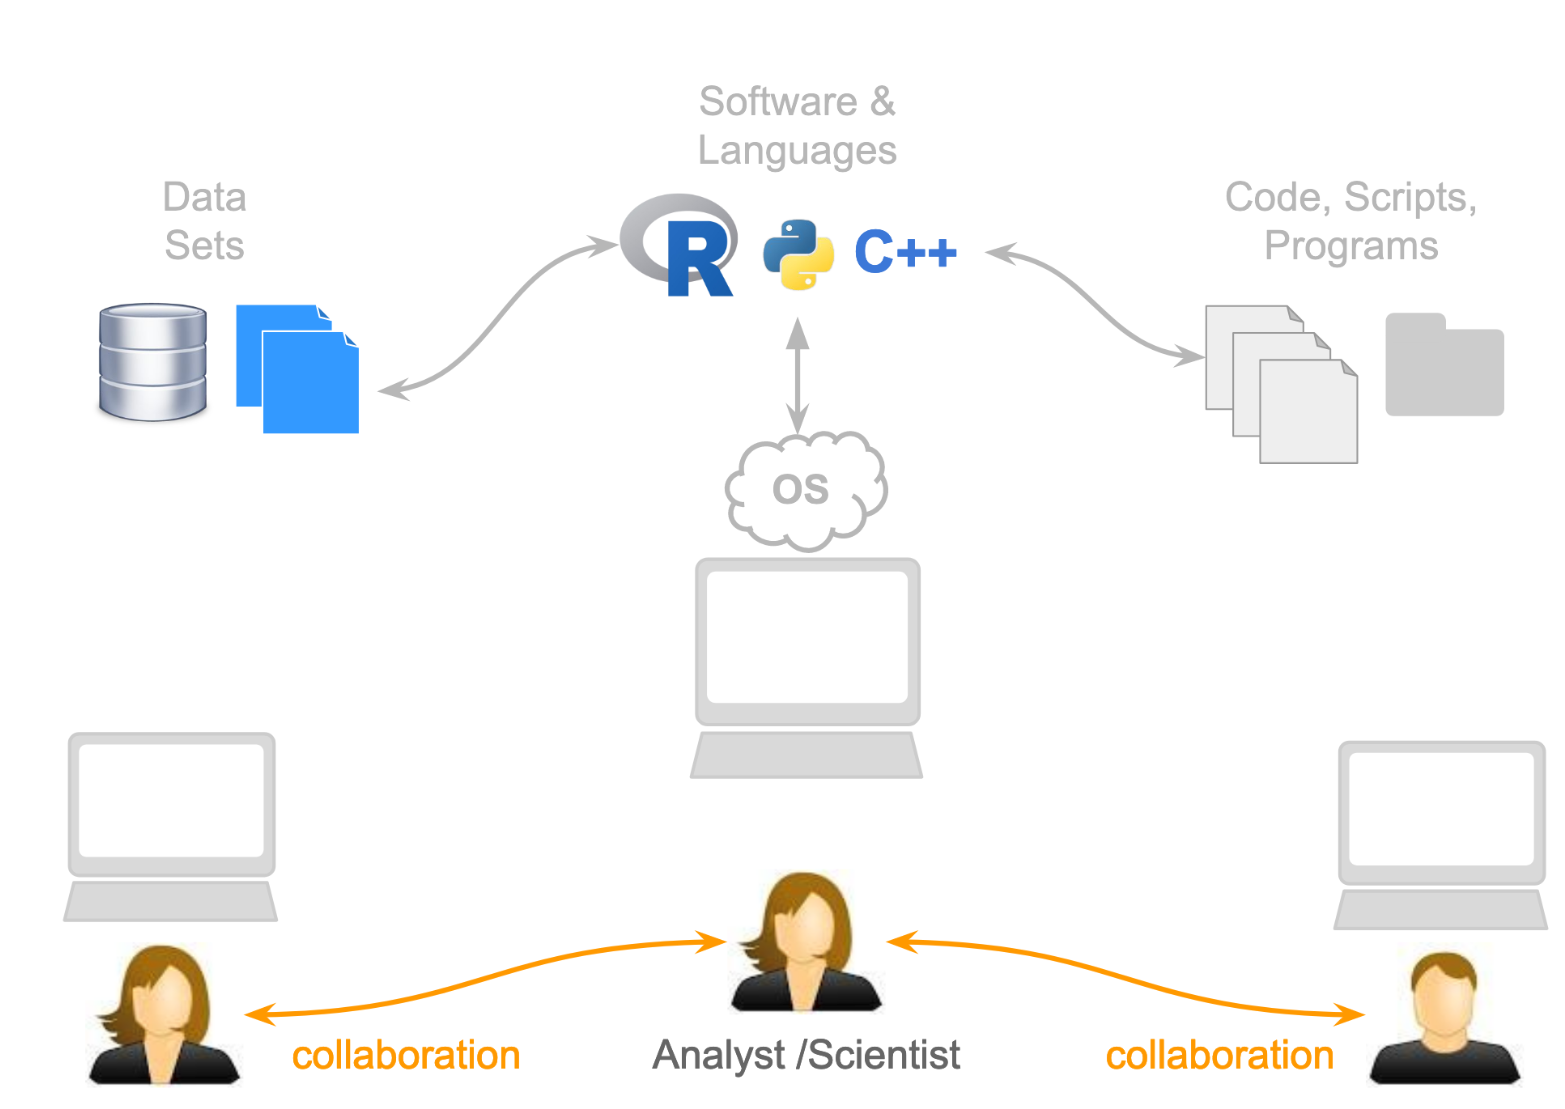
\includegraphics[scale=0.25]{sports_3.png}
\end{center}


\end{frame}
%--------------------------------------------
\begin{frame}
\frametitle{Statistics vs. Data Science}
%Nobody at this point will argue that Statistics is an important part of data science, but there some differences
\begin{itemize}
\item Statistics traditionally is concerned with analysing experimental data that have been
collected to explain and check the validity of specific hypothesis.
\item Data Science typically is concerned with  analysing observational data that have been 
collected for other reasons, not under control of the investigator, to create new ideas. Data Science involves The Big Picture.
% everything else that is surrounding the data itself
\end{itemize}
\begin{center}
\vspace{-.35cm}
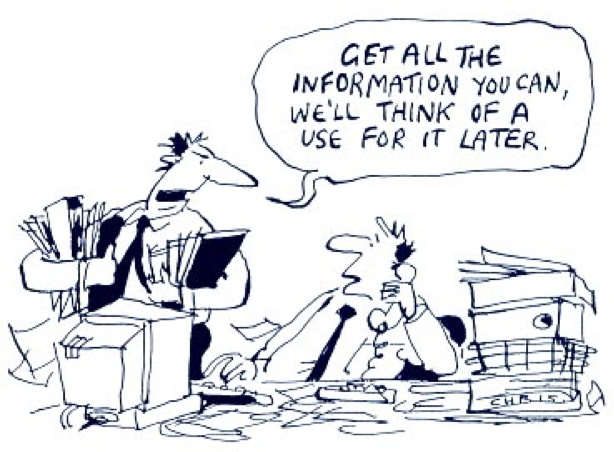
\includegraphics[scale=0.55]{ds.png}
\end{center}
% These two approaches of learning from data should be complementary
\end{frame}
%----------------------------------------------
\begin{frame}
\frametitle{Statistics}
\textcolor{blue}{Statistics} is the art and science of designing studies and analysing the data that those studies produce. 
Its ultimate goal is translating data into knowledge. Statistics is the art and science of learning from data.

\end{frame}
%----------------------------------------------
\section{The Data Analysis Cycle}
%----------------------------------------------
\begin{frame}
\frametitle{The Data Analysis Cycle}
\begin{center}
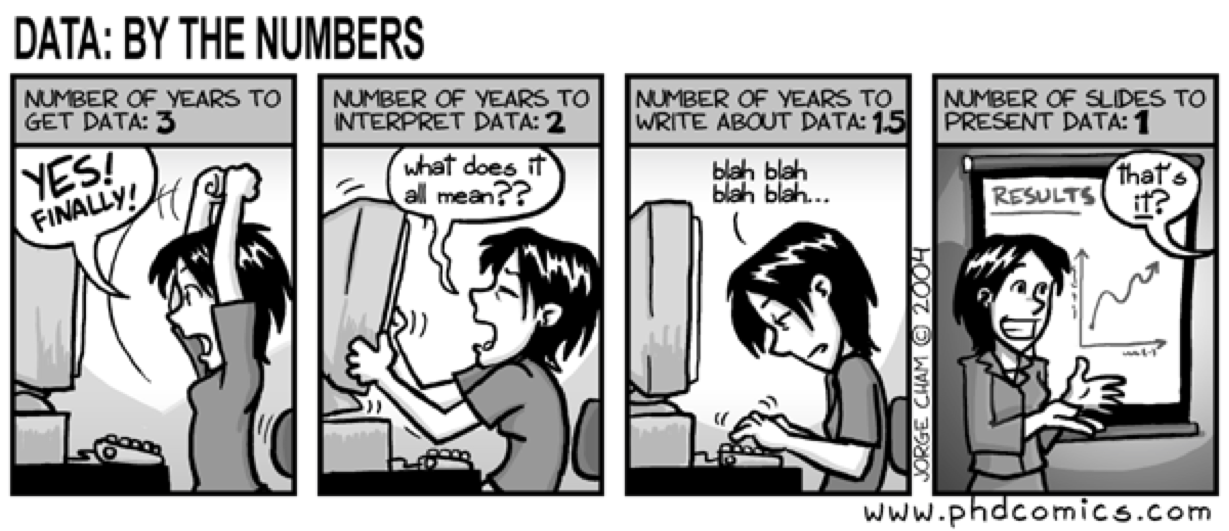
\includegraphics[scale=0.55]{comic.png}
\end{center}
% This is where analysis activities take place. In practice, this is where we spend most of our time. 
\end{frame}
%---------------------------------------------
%---------------------------------------------
\begin{frame}
\frametitle{The Data Analysis Cycle (I)}
\begin{columns}
    \column{0.55\textwidth}
    \hspace*{1cm}
    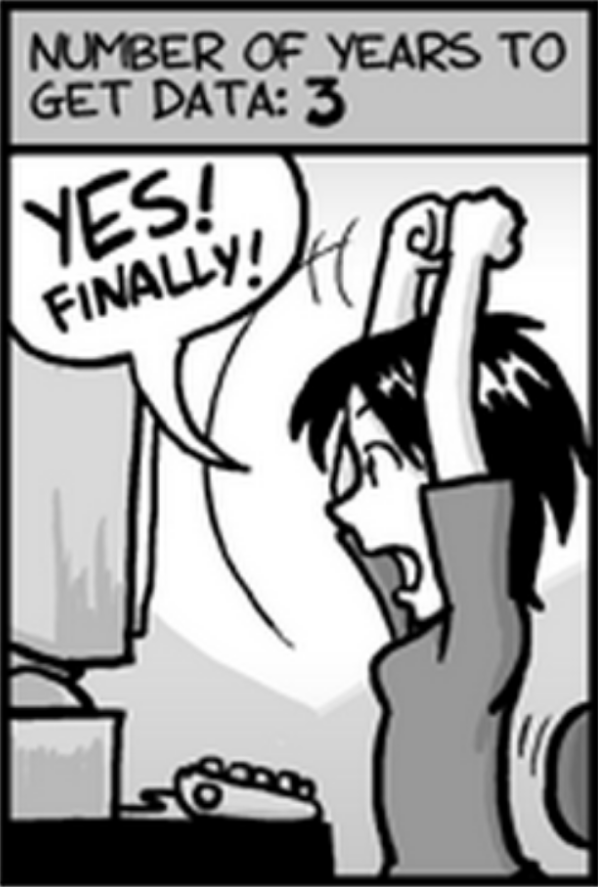
\includegraphics[scale=0.4]{im1.png}
    \column{0.5\textwidth}
 %    \hspace*{-1cm}
   %    \flushleft
    Data Preparation  
    \begin{itemize}
    \item[] Acquisition
    \item[] Storage
    \item[] Cleaning
    \item[] Processing
    \item[] Tidying
    \item[] Reshaping
    \item[] Wrangling
    \end{itemize}
\end{columns}
\end{frame}
%---------------------------------------------
\begin{frame}
\frametitle{The Data Analysis Cycle (II)}
\begin{columns}
    \column{0.55\textwidth}
    \hspace*{1cm}
    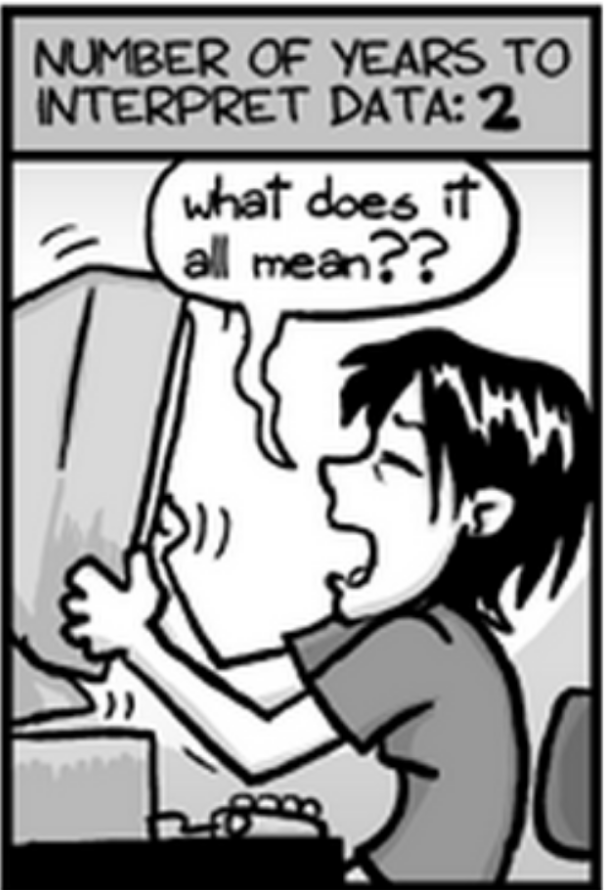
\includegraphics[scale=0.4]{im2.png}
    \column{0.5\textwidth}
 %    \hspace*{-1cm}
   %    \flushleft
    Core Data Analysis  
    \begin{itemize}
    \item[] Exploration
    \item[] Description
    \item[] Visualization
    \item[] Hypothesis Tests
    \item[] Inference
    \item[] Simulation
    \item[] Model Fitting
    \end{itemize}
\end{columns}
\end{frame}
%---------------------------------------------
\begin{frame}
\frametitle{The Data Analysis Cycle (III)}
\begin{columns}
    \column{0.55\textwidth}
    \hspace*{1cm}
    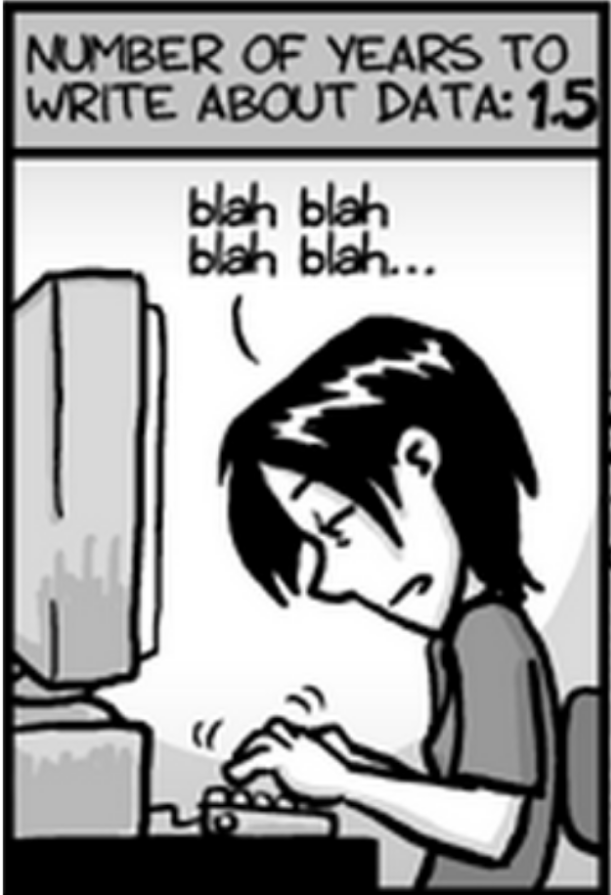
\includegraphics[scale=0.4]{im3.png}
    \column{0.5\textwidth}
 %    \hspace*{-1cm}
   %    \flushleft
    Reports  
    \begin{itemize}
    \item[] Document(s)
    \item[] Article(s)
    \item[] Book(s)
    \item[] Poster(s)
    \item[] Blog post(s)
    \item[] Dissertation
    \item[] News
    \end{itemize}
\end{columns}
\end{frame}
%---------------------------------------------
\begin{frame}
\frametitle{The Data Analysis Cycle (IV)}
\begin{columns}
    \column{0.55\textwidth}
    \hspace*{1cm}
    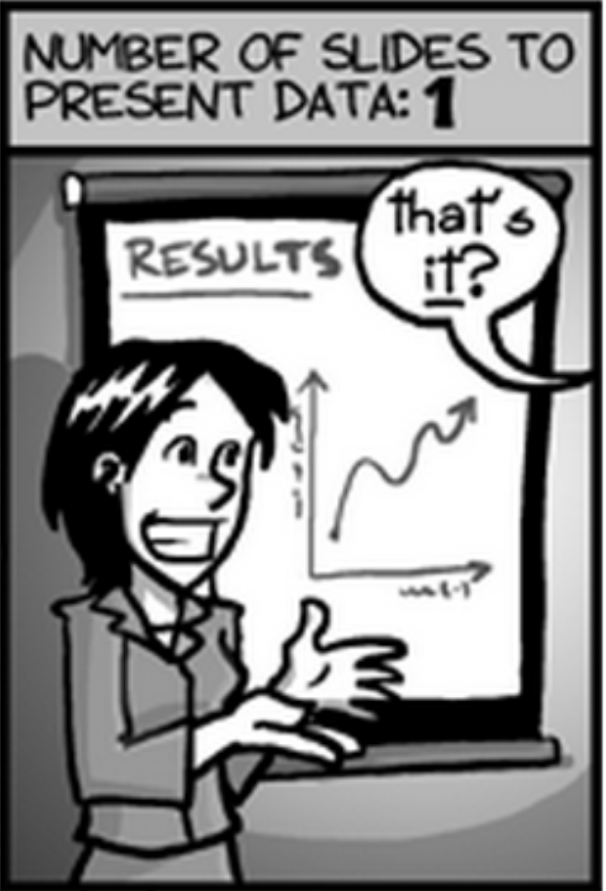
\includegraphics[scale=0.4]{im4.png}
    \column{0.5\textwidth}
 %    \hspace*{-1cm}
   %    \flushleft
    Communication  
    \begin{itemize}
    \item[] Oral
    \item[] Print
    \item[] Web
    \item[] Audio
    \item[] Tidying
    \item[] Video
    \item[] Other
    \end{itemize}
\end{columns}
\end{frame}
%---------------------------------------------
\begin{frame}
\frametitle{... not everything is Big Data and a black box}
Imagine $10$ people with $10,000$ blood pressure measurements on each of their two arms. It looks like $200,000$ observations.  But really there are only $10$ people. But a black box might not take proper account of the difference between $10$ subjects with $10,000$ observations each and $10,000$ subjects with $10$ observations each. Those are very different. We hope our statistical methods take account of this. 

\end{frame}
%---------------------------------------------
\begin{frame}
\frametitle{... be aware of the GIGO principle}

It is not possible to carry out an accurate statistical analysis of bad quality or inaccurate data. Read these  entries as an example. Flawed data and serious math errors made Tesla Autopilot look better (than it actually was). It also was a badly designed experiment to compare crash per million miles before the autosteering feature was activated and afterward. \\[10pt]
\begin{itemize}
\item \href{https://junkcharts.typepad.com/numbersruleyourworld/2019/03/excel-error-but-could-happen-in-any-tool.html}{\color{blue}{\underline{Entry 1}}}
\item \href{https://arstechnica.com/cars/2019/02/in-2017-the-feds-said-tesla-autopilot-cut-crashes-40-that-was-bogus/}{\color{blue}{\underline{Entry 2}}}
\end{itemize}
\end{frame}
%---------------------------------------------
\begin{frame}
\frametitle{Computational tool}
\begin{itemize}
\item The main computational tool will be the computing and programming environment R.
\item The main workbench I will be using is the IDE RStudio.
\end{itemize}
\end{frame}
%---------------------------------------------
%%%%
\end{document}
%%%%
